\section{سوال ششم}

در این تمرین می‌خواهیم با مدیریت حافظه اصلی در لینوکس آشنا شویم.

در لینوکس همه اطلاعات به‌صورت فایل ذخیره شده است. به‌طور مثال درون دایرکتوری \texttt{/proc} اطلاعات مربوط به هر پردازه و منابع سیستم موجود است. در این دایرکتوری، به ازای هر پردازه موجود در سیستم یک دایرکتوری با شماره PID آن پردازه ساخته شده است. که اطلاعات مربوط به آن پردازه را نگهداری می‌کند. همچنین اطلاعاتی مانند اطلاعات مربوط به حافظه اصلی و... را می‌توان در این دایرکتوری یافت.

محتوای این فایل را نمایش دهید.

برای اینکه ببینیم چقدر از حافظه اصلی استفاده شده است، از دستور \texttt{free} نیز می‌توان استفاده کرد.

\begin{qsolve}
	به دایرکتوری گفته شده می‌رویم و با دستور \texttt{meminfo cat} محتویات فایل را می‌خوانیم

	\begin{center}
		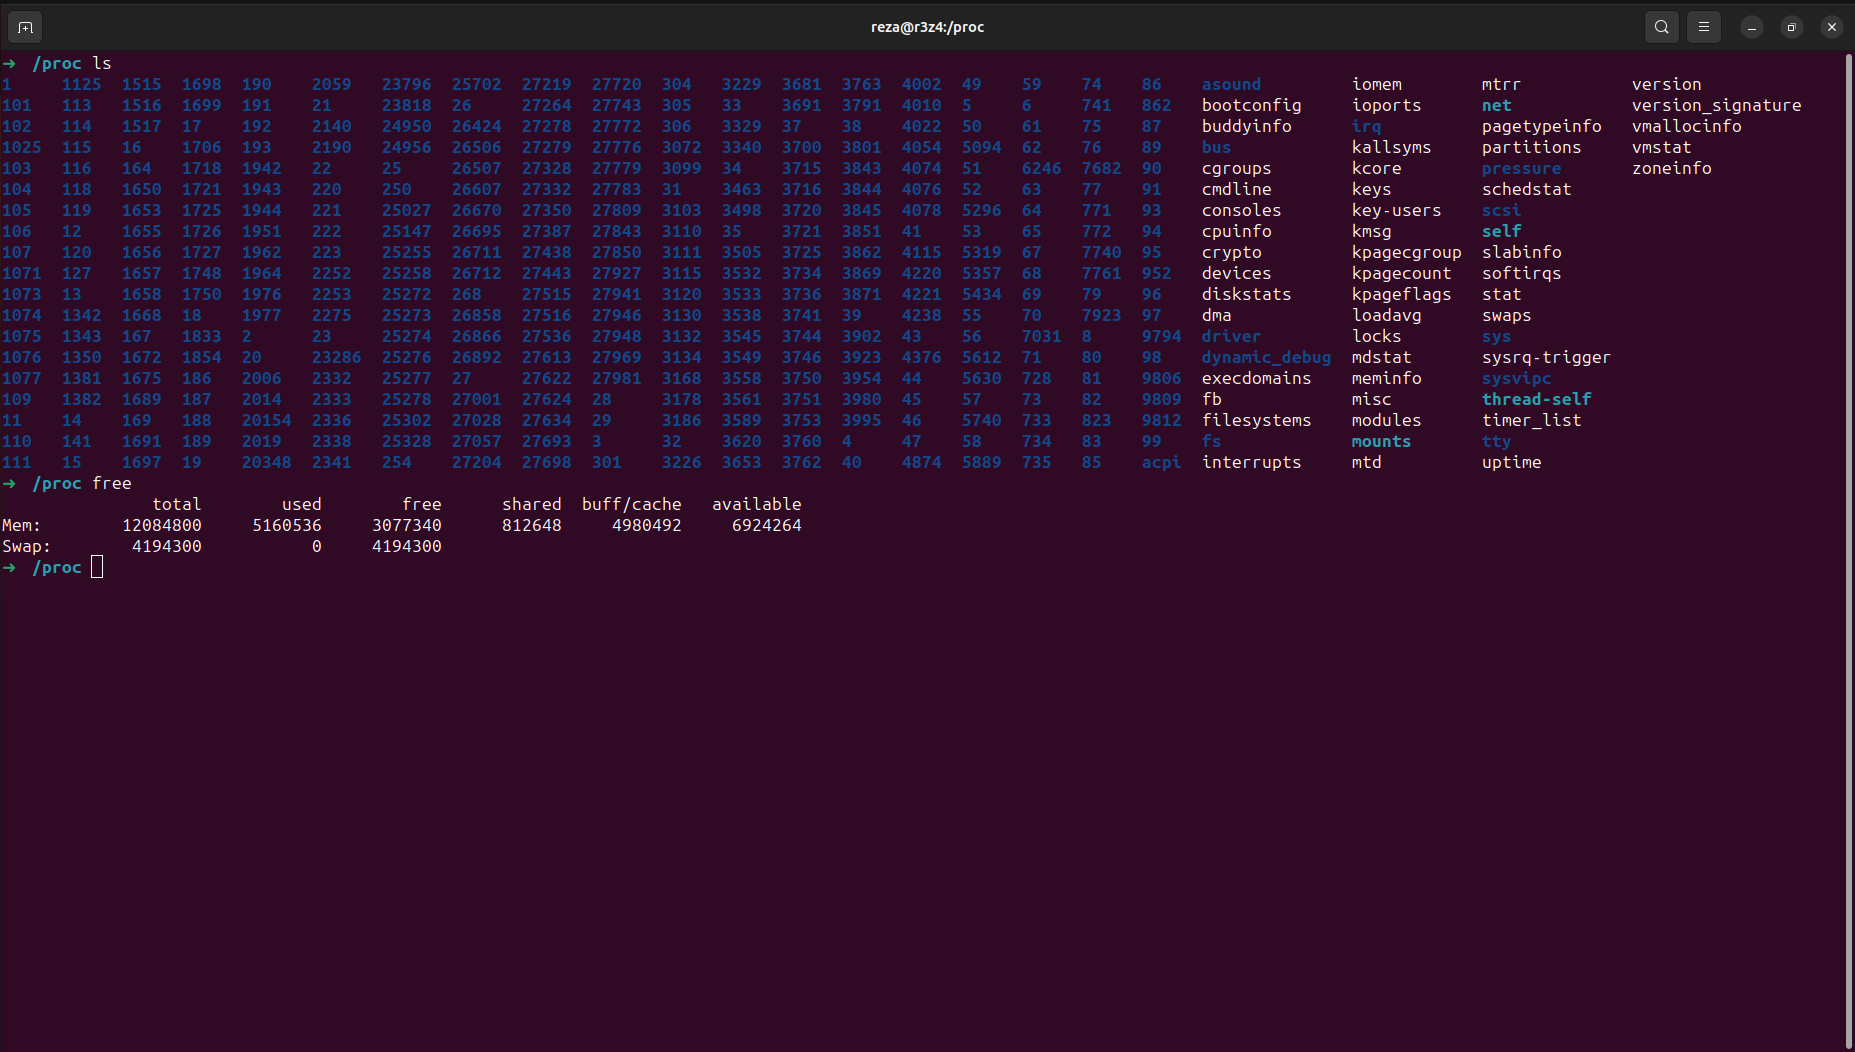
\includegraphics[width=\textwidth]{pics/img4.png}
	\end{center}
	
	\begin{center}
		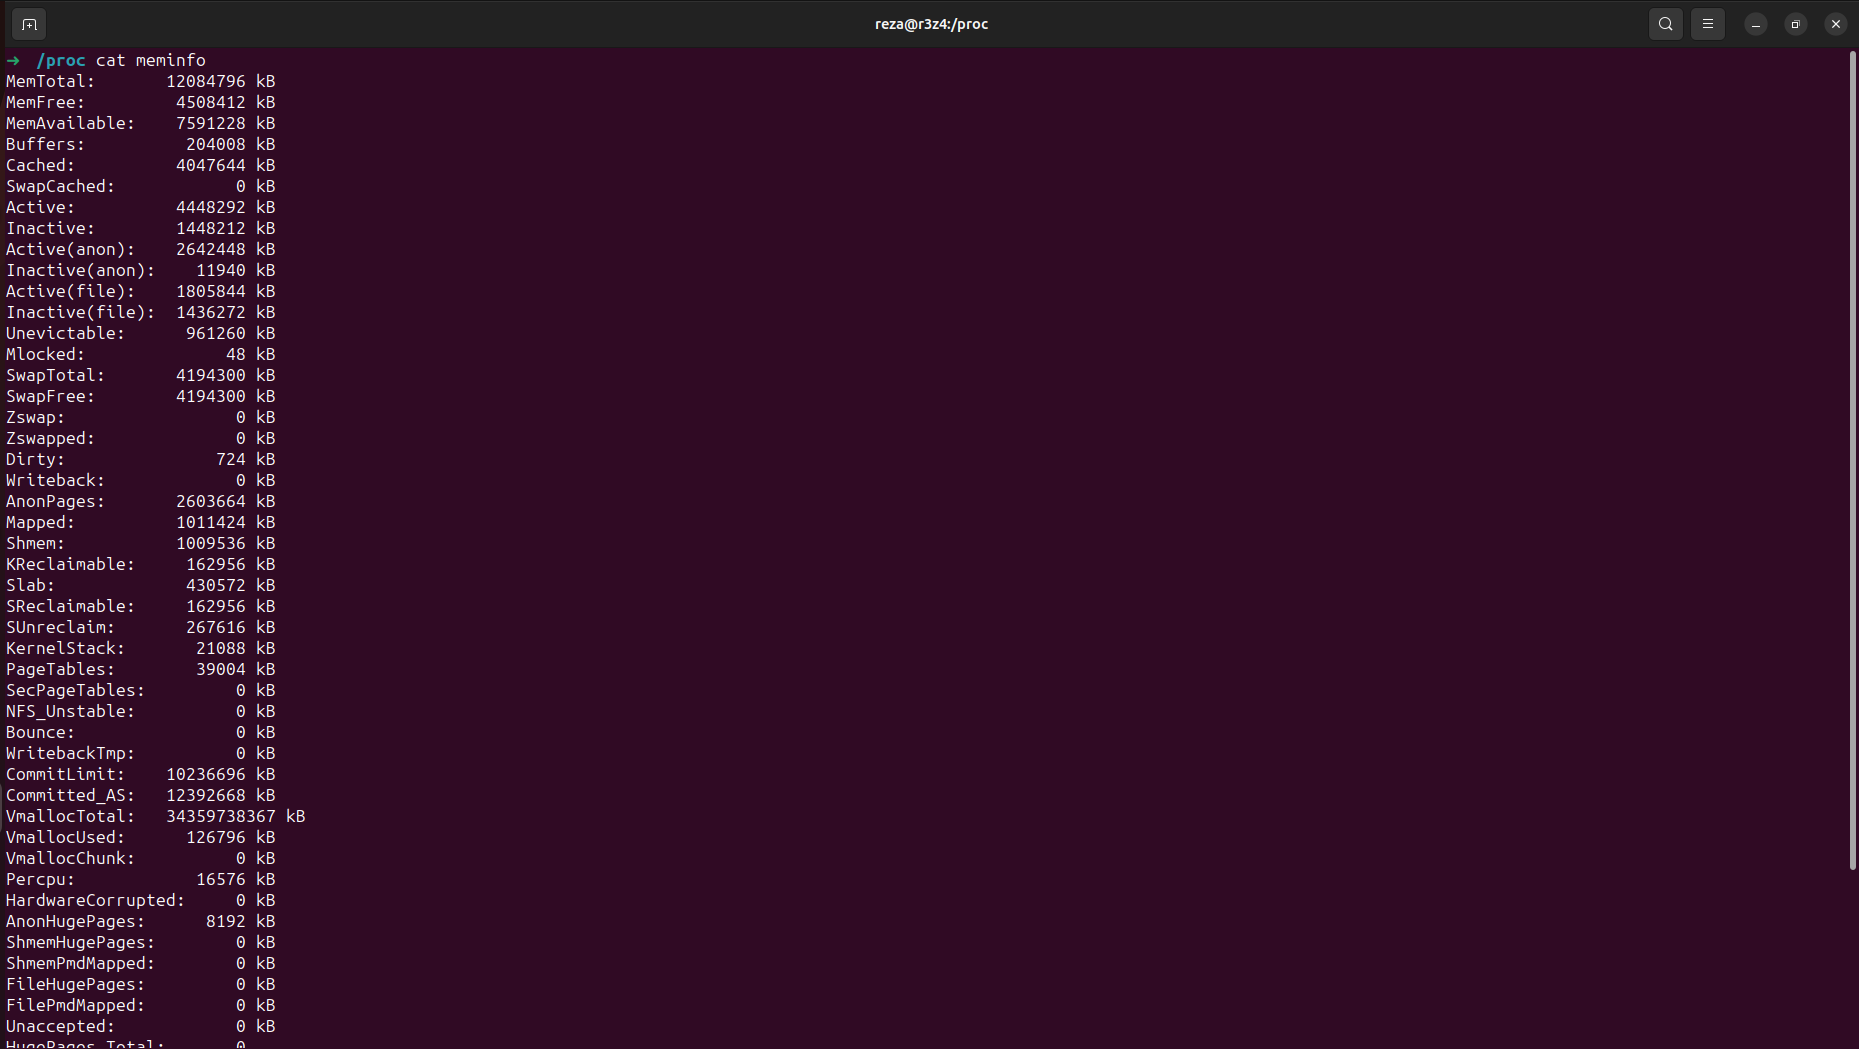
\includegraphics[width=\textwidth]{pics/img8.png}
	\end{center}
	
	در خروجی فایل \texttt{meminfo}، ستون‌های مختلف به معنای زیر هستند:
	
	


\end{qsolve}

\begin{qsolve}
	\begin{enumerate}
		\item :MemTotal مجموع حافظه اصلی سیستم به کیلوبایت.
		\item :MemFree مقدار حافظه اصلی خالی و در دسترس به کیلوبایت.
		\item :MemAvailable: مقدار حافظه اصلی در دسترس برای پراسس‌ها به کیلوبایت.
		\item :Buffers حافظه‌ای که برای نگهداری داده‌های برنامه‌های I/O استفاده می‌شود.
		\item :Cached حافظه‌ای که برای نگهداری داده‌هایی که توسط سیستم فایل‌های کش شده‌اند، استفاده می‌شود.
		\item :SwapCached حافظه‌ای که در بخش فایل‌های صفحه‌بندی (swap) برای فایل‌های کش شده استفاده شده است.
		\item :Active حافظه‌ای که در حال استفاده توسط فرآیندهای فعال است.
		\item :Inactive حافظه‌ای که در حال حاضر توسط فرآیندهای غیرفعال استفاده نمی‌شود.
		\item و...
	\end{enumerate}
	
	
	
		دستور \texttt{-h free} را اجرا کرده و توضیح دهید که هر یک از ستون‌های آن به چه معناست؟

خروجی دستور \texttt{-h free}:

\begin{center}
	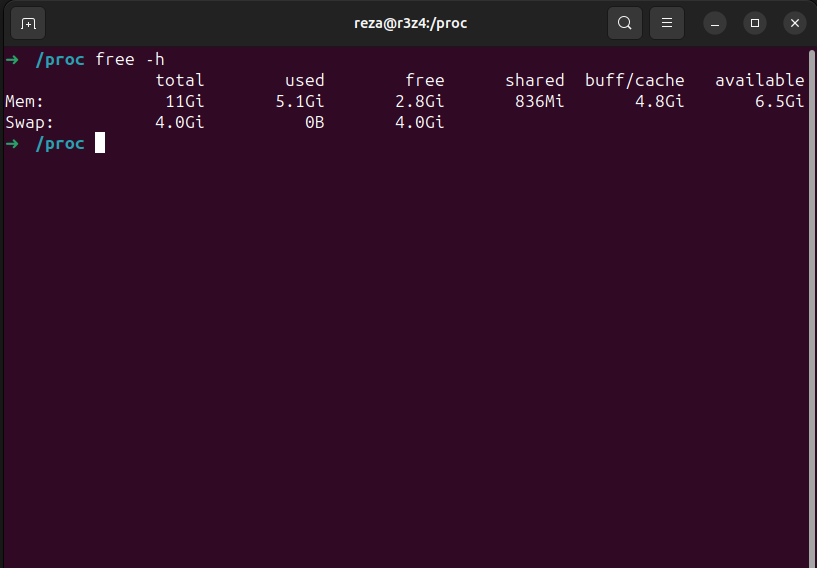
\includegraphics[width=10cm]{pics/img5.png}
\end{center}

با توجه به خروجی بالا، ستون‌های مختلف در دستور \texttt{free -h} به معنای زیر هستند:
\begin{enumerate}
	\item :total مجموع حافظه فیزیکی (RAM) و حافظه اصلی سیستم.
	\item :used مقداری از حافظه فیزیکی که در حال استفاده است.
	\item :free مقداری از حافظه فیزیکی که در حال حاضر خالی و در دسترس است.
	\item :shared حافظه فیزیکی مشترک بین پردازه‌ها.
	\item :buff/cache مقداری از حافظه فیزیکی که به عنوان بافر و کش استفاده می‌شود.
	\item :available حافظه فیزیکی در دسترس برای پراسس‌ها.
\end{enumerate}


\end{qsolve}



\begin{qsolve}
	
	برای اینکه تغییرات حافظه اصلی را دنبال کنیم، می‌توان از دستور \texttt{-h free watch} استفاده کرد.
	\begin{center}
		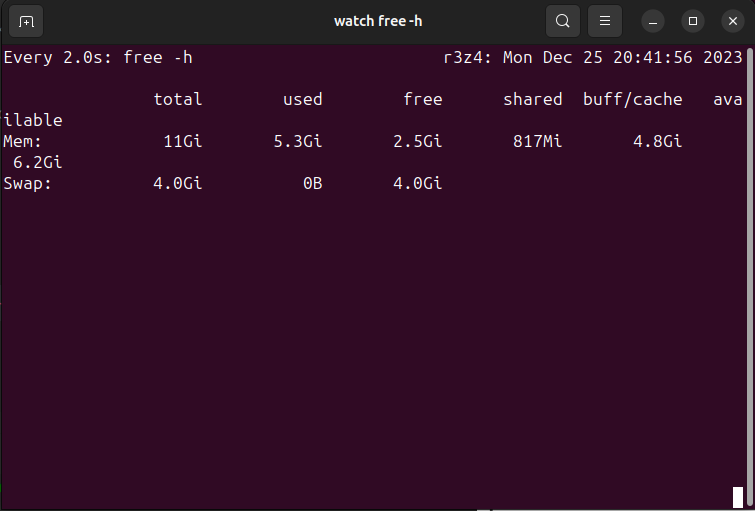
\includegraphics[width=10cm]{pics/img6.png}
	\end{center}
	
	
	
	همانطور که در خروجی دستور \texttt{free} می‌بینید، حجم زیادی از حافظه اصلی به بافر و \texttt{cache} اختصاص داده شده است. برای پاک کردن فضای اشغال شده توسط \texttt{cache} می‌توان از دستور زیر استفاده کرد.
	
	\begin{latin}
		\texttt{sudo sh -c "sync; echo 3 > /proc/sys/vm/drop\_caches}
	\end{latin}
	
	دستور فوق را تفسیر کنید و دوباره با دستور \texttt{free} مقدار ستون \texttt{buff/cache} را نشان دهید:
	
	\begin{center}
		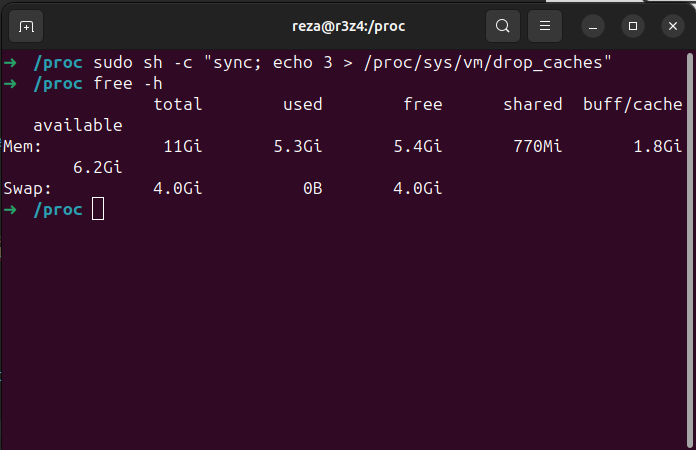
\includegraphics[width=10cm]{pics/img7.png}
	\end{center}
	
پس از اجرای دستور فوق، مقدار ستون \texttt{buff/cache} به \texttt{G 8.1}کاهش پیدا کرد.

تفسیر این دستور به صورت زیر است:
\begin{enumerate}
	\item \texttt{sudo}: استفاده از دستورات با دسترسی ادمین .(superuser)
	\item \texttt{-c sh}: اجرای یک دستور شل
	\item \begin{latin}
		\texttt{"sync; echo 3 > /proc/sys/vm/drop\_caches"} 
	\end{latin}
	
	در این بخش، دو دستور اجرا می‌شود. ابتدا دستور \texttt{sync} اجرا می‌شود که اطلاعات موجود در حافظه نهان (cache) را بر روی دیسک ذخیره می‌کند. سپس دستور
	
	 \begin{latin}
	 	\texttt{echo 3 > /proc/sys/vm/drop\_caches}
	 \end{latin}
	  اجرا می‌شود که باعث پاک شدن محتوای حافظه نهان (cache) می‌شود. عدد 3 به معنای پاک کردن بخش‌های ،cache مشترک و inode است.
\end{enumerate}
	
\end{qsolve}


